%% Based on a TeXnicCenter-Template by Gyorgy SZEIDL.
%%%%%%%%%%%%%%%%%%%%%%%%%%%%%%%%%%%%%%%%%%%%%%%%%%%%%%%%%%%%%

%------------------------------------------------------------
%
\documentclass{article}%
%Options -- Point size:  10pt (default), 11pt, 12pt
%        -- Paper size:  letterpaper (default), a4paper, a5paper, b5paper
%                        legalpaper, executivepaper
%        -- Orientation  (portrait is the default)
%                        landscape
%        -- Print size:  oneside (default), twoside
%        -- Quality      final(default), draft
%        -- Title page   notitlepage, titlepage(default)
%        -- Columns      onecolumn(default), twocolumn
%        -- Equation numbering (equation numbers on the right is the default)
%                        leqno
%        -- Displayed equations (centered is the default)
%                        fleqn (equations start at the same distance from the right side)
%        -- Open bibliography style (closed is the default)
%                        openbib
% For instance the command
%           \documentclass[a4paper,12pt,leqno]{article}
% ensures that the paper size is a4, the fonts are typeset at the size 12p
% and the equation numbers are on the left side
%
\usepackage{amsmath}%
\usepackage{amsfonts}%
\usepackage{amssymb}%
\usepackage{graphicx}
\usepackage[T1]{fontenc}
\usepackage[utf8]{inputenc}

\usepackage{rotating}
\usepackage{listings}
\usepackage{authblk}
\usepackage{float}
\usepackage{url}
\usepackage[unicode=true,
 bookmarks=true,bookmarksnumbered=false,bookmarksopen=false,
 breaklinks=false,pdfborder={0 0 1},backref=false,colorlinks=false]
 {hyperref}
%-------------------------------------------
\newtheorem{theorem}{Theorem}
\newtheorem{acknowledgement}[theorem]{Acknowledgement}
\newtheorem{algorithm}[theorem]{Algorithm}
\newtheorem{axiom}[theorem]{Axiom}
\newtheorem{case}[theorem]{Case}
\newtheorem{claim}[theorem]{Claim}
\newtheorem{conclusion}[theorem]{Conclusion}
\newtheorem{condition}[theorem]{Condition}
\newtheorem{conjecture}[theorem]{Conjecture}
\newtheorem{corollary}[theorem]{Corollary}
\newtheorem{criterion}[theorem]{Criterion}
\newtheorem{definition}[theorem]{Definition}
\newtheorem{example}[theorem]{Example}
\newtheorem{exercise}[theorem]{Exercise}
\newtheorem{lemma}[theorem]{Lemma}
\newtheorem{notation}[theorem]{Notation}
\newtheorem{problem}[theorem]{Problem}
\newtheorem{proposition}[theorem]{Proposition}
\newtheorem{remark}[theorem]{Remark}
\newtheorem{solution}[theorem]{Solution}
\newtheorem{summary}[theorem]{Summary}
\newenvironment{proof}[1][Proof]{\textbf{#1.} }{\ \rule{0.5em}{0.5em}}

\begin{document}

\title{A Topic Modeling Approach for Web Service Annotation}
\author[1]{Leandro Ordonez-Ante\thanks{leandro@unicauca.edu.co}}
\author[2]{Ruben Verborgh\thanks{ruben.verborgh@ugent.be}}
\author[1]{Juan Carlos Corrales\thanks{jcorral@unicauca.edu.co}}
\affil[1]{Grupo de Ingeniería Telemática (GIT), Universidad del Cauca
\\Calle 5 No 4-70, Popayán, Colombia}
\affil[2]{Multimedia Lab, Ghent University
\\Gaston Crommenlaan 8/102, 9050 Ghent, Belgium}

\renewcommand\Authands{ and }
\date{April 9, 2014}
\maketitle

\begin{abstract}

\end{abstract}
\section{Introduction}
\label{sec:introduction}

\noindent During the last two decades we have been witnessing how the Web has evolved from being a text and image repository on its early stages, to provide a huge offer of both information-providing and world-altering services. The current Web has posed a paradigm that revolutionized the generation and consumption dynamics of this kind of resources, encouraging its users, not merely to consume these services, but also to build and publish them.

This dominant paradigm of the current Web, has inspired the conception of initiatives into other communities such as the Telco providers, which include the GSMA’s One API \cite{GSMA:2013}, and the ECMA-348 \cite{ECMA:2012} and ECMA-323 \cite{ECMA:2011} standards. Such initiatives promote for network operators to expose their capabilities and information via Web service interfaces, easing this way for users (service designers and developers) to create and deploy new telecom services, with a reduced time-to-market and tailored to their specific needs.

Thus, the service offering inside the Web is diversifying and steadily growing, so it is necessary to provide the users with increasingly intelligent mechanisms for services search and retrieval, identifying in a truthful way the functionality provided by such resources while being able to deliver relevant services to the customer. The above has meant the transition from the traditional keyword-based or table-based search methods \cite{Bernstein:2002}, to approaches supported on semantic Web technologies which provide meaning for both the services specifications, and user queries, through a formal and machine-readable specification of knowledge (e.g. ontologies, taxonomies, lexical database and so on).

In practical terms, however, the actual implementation of semantic-based mechanisms for service retrieval has been restricted precisely due to the expensive procedure involved in the formal specification of services. Such a procedure comprises a time-consuming task of semantic annotation, performed by hand by service developers, who additionally require specialized knowledge on models for semantic description of services (e.g. OWL-S, WSMO, SAWSDL), as well as the aforementioned formal specifications of knowledge.

In order to overcome this limitation, currently some approaches are considered to tackle the problem of semantic service annotation, by applying knowledge discovery and emergent semantics techniques over a huge corpus of service descriptors, which in some cases already contains annotations made by consumers in a collaborative way. Those approaches however, has serious limitations in terms of the reliability of the users feedback they are built upon, which impacts the precision of search and selection tasks. Therefore it’s considered necessary to develop mechanisms that enable the automation of semantic service annotation tasks.

This paper introduces our proposal for service annotation, based on processing existing web service documentation resources for extracting information regarding its offered capabilities. By uncover the hidden semantic structure of such information through statistical analysis techniques, we are able to associate meaningful annotations to the services operations, and to group those operations into non-exclusive semantic related categories.

Based on this approach we have build Topicalizer, a tool that allows the user to process a bunch of SOAP API descriptors (WSDL documents), in order to group the technical information they contain into semantic categories, and specifying such categorization as RDF statements stored in a Sesame triple-store, to which users may access and issue SPARQL queries.
\section{Motivation and Background}

\noindent The Web is emerging as a medium for connecting distributed applications, becoming---more than an information system---into a platform that
supports the operation of a huge ecosystem of services \cite{Webber:2010a}, which are built under different architectures and design philosophies. Leonard Richardson has proposed in \cite{Richardson:2008} a schema for classifying services on the Web, defining three maturity levels (plus a zero level). Each of the levels represents one element of what Richardson calls \emph{the technology stack for web services}: URI, HTTP, Hypermedia (see Figure \ref{richardsonModel}). This way, services are classified according to the technologies that supports their operation.

\begin{figure}[H]
\center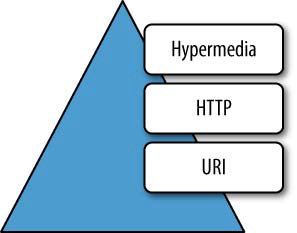
\includegraphics[scale=0.7]{images/WS-MaturityModel}

\caption{Rchardson's service maturity model. {\scriptsize source: \cite{Webber:2010a}}}
\label{richardsonModel}
\end{figure}

\begin{itemize}
\item \emph{Level zero services}: services at this level are characterized by having an unique URI and using only one HTTP method (typically \texttt{POST}). At this level there we find the XML-RPC services \cite{Laurent:2001} and most of the SOAP services. 
\item \emph{Level one services (URI support)}: At this level, services employ various URIs but only one HTTP method. In contrast to level zero services---which tunnel all the interactions through a unique and rather complex resource---services at level one expose multiple logical resources. However services at this level tunnel their actions by inserting parameters and values into a URI, which is then transmitted to a remote service (via \texttt{HTTP GET} typically). According to Richardson, most of the services out there that claim to be RESTful are actually level one services.
\item \emph{Level two services (HTTP support)}: this level deals with services that host many resources, each of which is addressable through its own URI. Additionally level two services support various HTTP methods on their resources. This level includes CRUD-like (\emph{Create}, \emph{Read}, \emph{Update}, \emph{Delete}) services, such as the Amazon cloud storage system (\emph{Amazon S3}: \href{http://aws.amazon.com/es/s3/} {http://aws.amazon.com/es/s3/}).
\item \emph{Level three services (Hypermedia support)}: At this level, we find real RESTful services: those having the features of level two services, plus supporting the notion of \emph{hypermedia as the engine of application state} (HATEOAS), that is to say, the representations of the resources hosted by the service contain controls that enable consumers to access related resources. This way the service leads its users through a trail of resources, causing application state changes in consequence. Examples of this kind of services include the Web (see section \ref{sub:The-Web-according}) and the REST API of \emph{Netflix} (\href{http://developer.netflix.com/docs/REST_API_Conventions} {http://developer.netflix.com/docs/REST\_{}API\_{}Conventions}). 
\end{itemize}

A research conducted by Maleshkova et al. \cite{Maleshkova:2010} reports that, despite the apparent spreading of RESTful services in the Web, there are actually few services that supports all the tenets and constraints of REST. The authors of this study have analyzed by hand 222 web APIs, randomly chosen from the \emph{Programmable Web }API directory\emph{} \footnote{Available at:\emph{ }\href{http://www.programmableweb.com/}{http://www.programmableweb.com/}}. The results that arose from their analysis, evidence that only 32\% of services could be considered---at least approximately---REST services (i.e., services from levels two and three in the Richardson maturity model), while the remaining 68\% was RPC and hybrid services (i.e., services from levels zero and one, according to the same model).

The study of Maleshkova also states that service development is driven by the particular criteria of its creators, rather than well-established standards and rules. Similarly, service documentation (specially REST service documentation) is not supported on interface description languages such as WSDL, but it is provided as HTML documents, which have no regular or standard structure. Therefore, the use of web services requires a cumbersome manual process which additionally hinders the execution of discovery, composition and invocation procedures. In this regard, some initiatives have been fostered, seeking the definition of standard formats for describing REST services. That is the case of WADL (\emph{Web Application Description Language}) \cite{W3C:2009}, a language intended for specifying HTTP-based web services and applications.

A WADL descriptor (or contract) is a document that specifies the set resources hosted by a service, as well as their associated URI templates, the HTTP methods the service supports and the representations it is able to receive and deliver. Just like WSDL, WADL enables automatic building of services clients, making them easier to consume and accessible to developers. Nonetheless, WADL descriptors merely describe the static view of services and applications, neglecting the user-resources interaction dynamics, which is better specified by hypermedia and media types. Consequently, as stated in \cite{Webber:2010b}, this kind of descriptor is suitable only for CRUD-like REST services (Level two services) whose functionality is limited to manipulate records from a data set.

So far, WADL has been poorly adopted as description language for REST services. Instead other studies have been conducted for defining service descriptors that include semantic metadata, which aim to enable the automatic discovery and composition of services. Semantic annotations make it possible for intelligent agents to understand the services functionality, and establishing service relationships at the semantic level (e.g., similarity, partial matching, and membership\cite{Paolucci:2002}).

In this regard the academic community has came up with proposals like hRESTS \cite{Kopecky:2008}\textemdash{}an HTML-based description microformat that allows specifying the services functional attributes, like its operations, inputs and outputs\textemdash{}, along with its extensions SA-REST \cite{Sheth:2007} and MicroWSMO \cite{Kopecky:2009}, which enable the semantic annotation of hREST descriptors.

Another approach to REST API description is \emph{RESTdesc}, proposed by Verborgh et al. in \cite{Verborgh:2013,Verborgh:2012a,Verborgh:2012b}. RESTdesc provides a functionality-centered format for semantic description of REST services, as well as an automatic discovery mechanism based on inference with logic rules specifying the capabilities of these resources. According to the authors of RESTdesc, the approach they propose is supported on well known technologies such as HTTP and RDF/Notation3 \cite{BernersLee:2011} and is grounded on the hypermedia and \emph{Linked Data} \cite{Bizer:2009} concepts, from which defines and leverages relationships between different services specifications, enabling intelligent agents to automatically discover and compose services.

Finally, the approach addressed by Saquicela et al. in \cite{Saquicela:2010}, introduces a proposal for semantic description of REST services which allows their storage and invocation, as well as an automatic technique for semantic annotation of service parameters, supported on the DBpedia ontology\cite{Auer:2007} and external resources such as suggestion and synonyms services.

Since, in general terms, there is a sort of barrier regarding the adoption of new formats for specifying the web service semantics, the proposal conceived under my master's degree work entitled \textquotedblleft{}\emph{Automated semantic annotation of services on the Web}\textquotedblright{}, intends to use the information currently available in service description documents---i.e., WSDL interfaces for SOAP services and HTML documents for XML-RPC and REST services---in order to abstract a knowledge representation based on the content of such documentation, from which it would be possible to establish semantic similarity relations between services. This proposal is founded on three main processes: 

\begin{enumerate}
\item Extraction of technical information related to service functionality. 
\item Analysis of the extracted information for identifying conceptual categories
the services they comprise. 
\item Deriving a taxonomy from the categories obtained in process (2). 
\end{enumerate}

% Nowadays the amount of information and resources available on the Web is huge and ever increasing, so that it has exceeded our ability for locating and accessing the resources we need. This way, increasingly sophisticated computational tools are required for organizing, searching and understanding those resources, beyond the traditional information indexing and retrieval approaches.
% 
% Semantic annotation, is one of the core concepts of the current proposal. It aims to make explicit for machines, the meaning (the semantics) of content and resources available in large repositories of information. This latter constitutes one of the requirements to meet to finally materializing the Semantic Web. The semantic annotation procedure is commonly supported in formal representation of knowledge, as the aforementioned ontologies, and for services, consists in associating ontological entities to the terms defining the attributes of the service in its descriptor document [8], allowing for instance, for service search engines to effectively comprehend (on a semantic level) both the services functionality as the service’s  clients requests, enabling them to accurately respond to service inquiries.
% 
% Traditionally, this semantic annotation procedure must be performed by hand by service designers and developers or in a collaborative way by service users (conceiving a sort of folksonomy of services). In both cases, the large and growing amount of services, along with the lack of knowledge regarding semantic description methods for services and the scarceness of suitable domain ontologies, has overwhelmed the human ability for performing this semantic annotation task. Additionally, the human intervention in marking up the services descriptors with ontological entities involves a very expensive process in terms of time, effort and resources. In this regard, the focus of the present approach is on leveraging current techniques taken from the fields of machine learning, information retrieval and knowledge discovery, for automating the semantic annotation of web services. The next section will deal the revision of some previous works regarding the problem being tackled herein.
\section{Related Work}
\label{sec:related_work}

\noindent At the end of the last section we reviewed some works regarding REST APIs description. This section continues with that review but focuses on works addressing semantic annotation of Web services and resources in general.

In \cite{Loutas:2010} Loutas et al. explore alternative approaches for semantic annotation of available services and resources in the Web. In this work the author conceive information constructs derived from collaborative tagging systems (also known as folksonomies) as specifications of shared knowledge, which may be suitable for associate semantic annotations to service interfaces. However, as stated by Martinez-Cruz et al. in \cite{MartinezCruz:2010}, the wide-open nature of folksonomies involves some shortcomings in terms of organizing, searching and retrieval of resources based on tags, due to its lack of formal semantics. That way, the authors of \cite{MartinezCruz:2010} propose to build an \textit{ontology-based semantic layer} on top of these collaborative tagging systems to formalize the knowledge gathered within them. 

In other related work by Loutas et al. \cite{Loutas:2012}, they introduce a proposal for a search engine for web services, which operates on service descriptors specified in SA-REST or SAWSDL. In order to deal with heterogeneous service description formats, the authors define a comprehensive \textit{Reference Service} model to which all the crawled services are mapped. The main shortcoming of this approach lies on the fact that it operates on semantic description formats whose adoption is rather limited.

The approach outlined in \cite{Azmeh:2010} by Azmeh et al. pose the use of techniques of machine learning such as Formal Concept Analysis (FCA) and Relational Concept Analysis (RCA), for extracting and representing the technical information contained in service descriptors as conceptual hierarchies. However, the approach introduced in this work is not that exhaustive when it comes to identify similarity between services, since it relies on syntactic comparison of the terms comprising the service interfaces (i.e. WSDLs). 

The approach we propose contributes towards automating the process of semantic annotation of web services descriptors, by combining techniques of text mining and unsupervised machine learning (i.e. Latent Dirichlet Allocation–LDA) for enabling  automatic and incremental generation of a formal model of knowledge from existing service documentation sources. Such model is meant to be used in annotating and categorizing services operations, through a platform that implements the above techniques. 

Next section will address the description of our proposal, by outlining each one of the three processes stated at the end of section \ref{sec:motivation_background}.

\section{Proposal}

\noindent 

\section{Experimentation}
\label{sec:experimentation}

\noindent In order to assess the feasibility of our proposal we build a prototype called \emph{Topicalizer}, which implements the mechanisms described throughout this report, for the particular case of SOAP services. 

The implemented system receives as input a list of URIs from real WSDL interfaces available online. The system retrieves each WSDL and processes it by following the techniques outlined in sections \ref{subsub:soap} and \ref{subsub:Service-documentation-cleaning} and stores its relevant information into a service registry. In running this process, a stream of documents is generated, each one of them containing information related to a specific SOAP service operation. Then the stream of documents is categorized based on the document's content by applying the \emph{online LDA} algorithm as described in sections \ref{subsub:The-Latent-Dirichlet} and \ref{subsub:Application-of-LDA}. Such categorization arranges semantically-related documents into clusters which are defined by a weighted set of terms, that in turn become annotations on the operations that each document represents. The information gathered from the categorization process is specified in RDFS---conforming to the data model defined in section \ref{subsub:RDF-spec-of-KNOWEB}---and stored into an RDF triplestore.

The system architecture is depicted in Figure \ref{prototype-architecture}:

\begin{figure}
\begin{center}
 
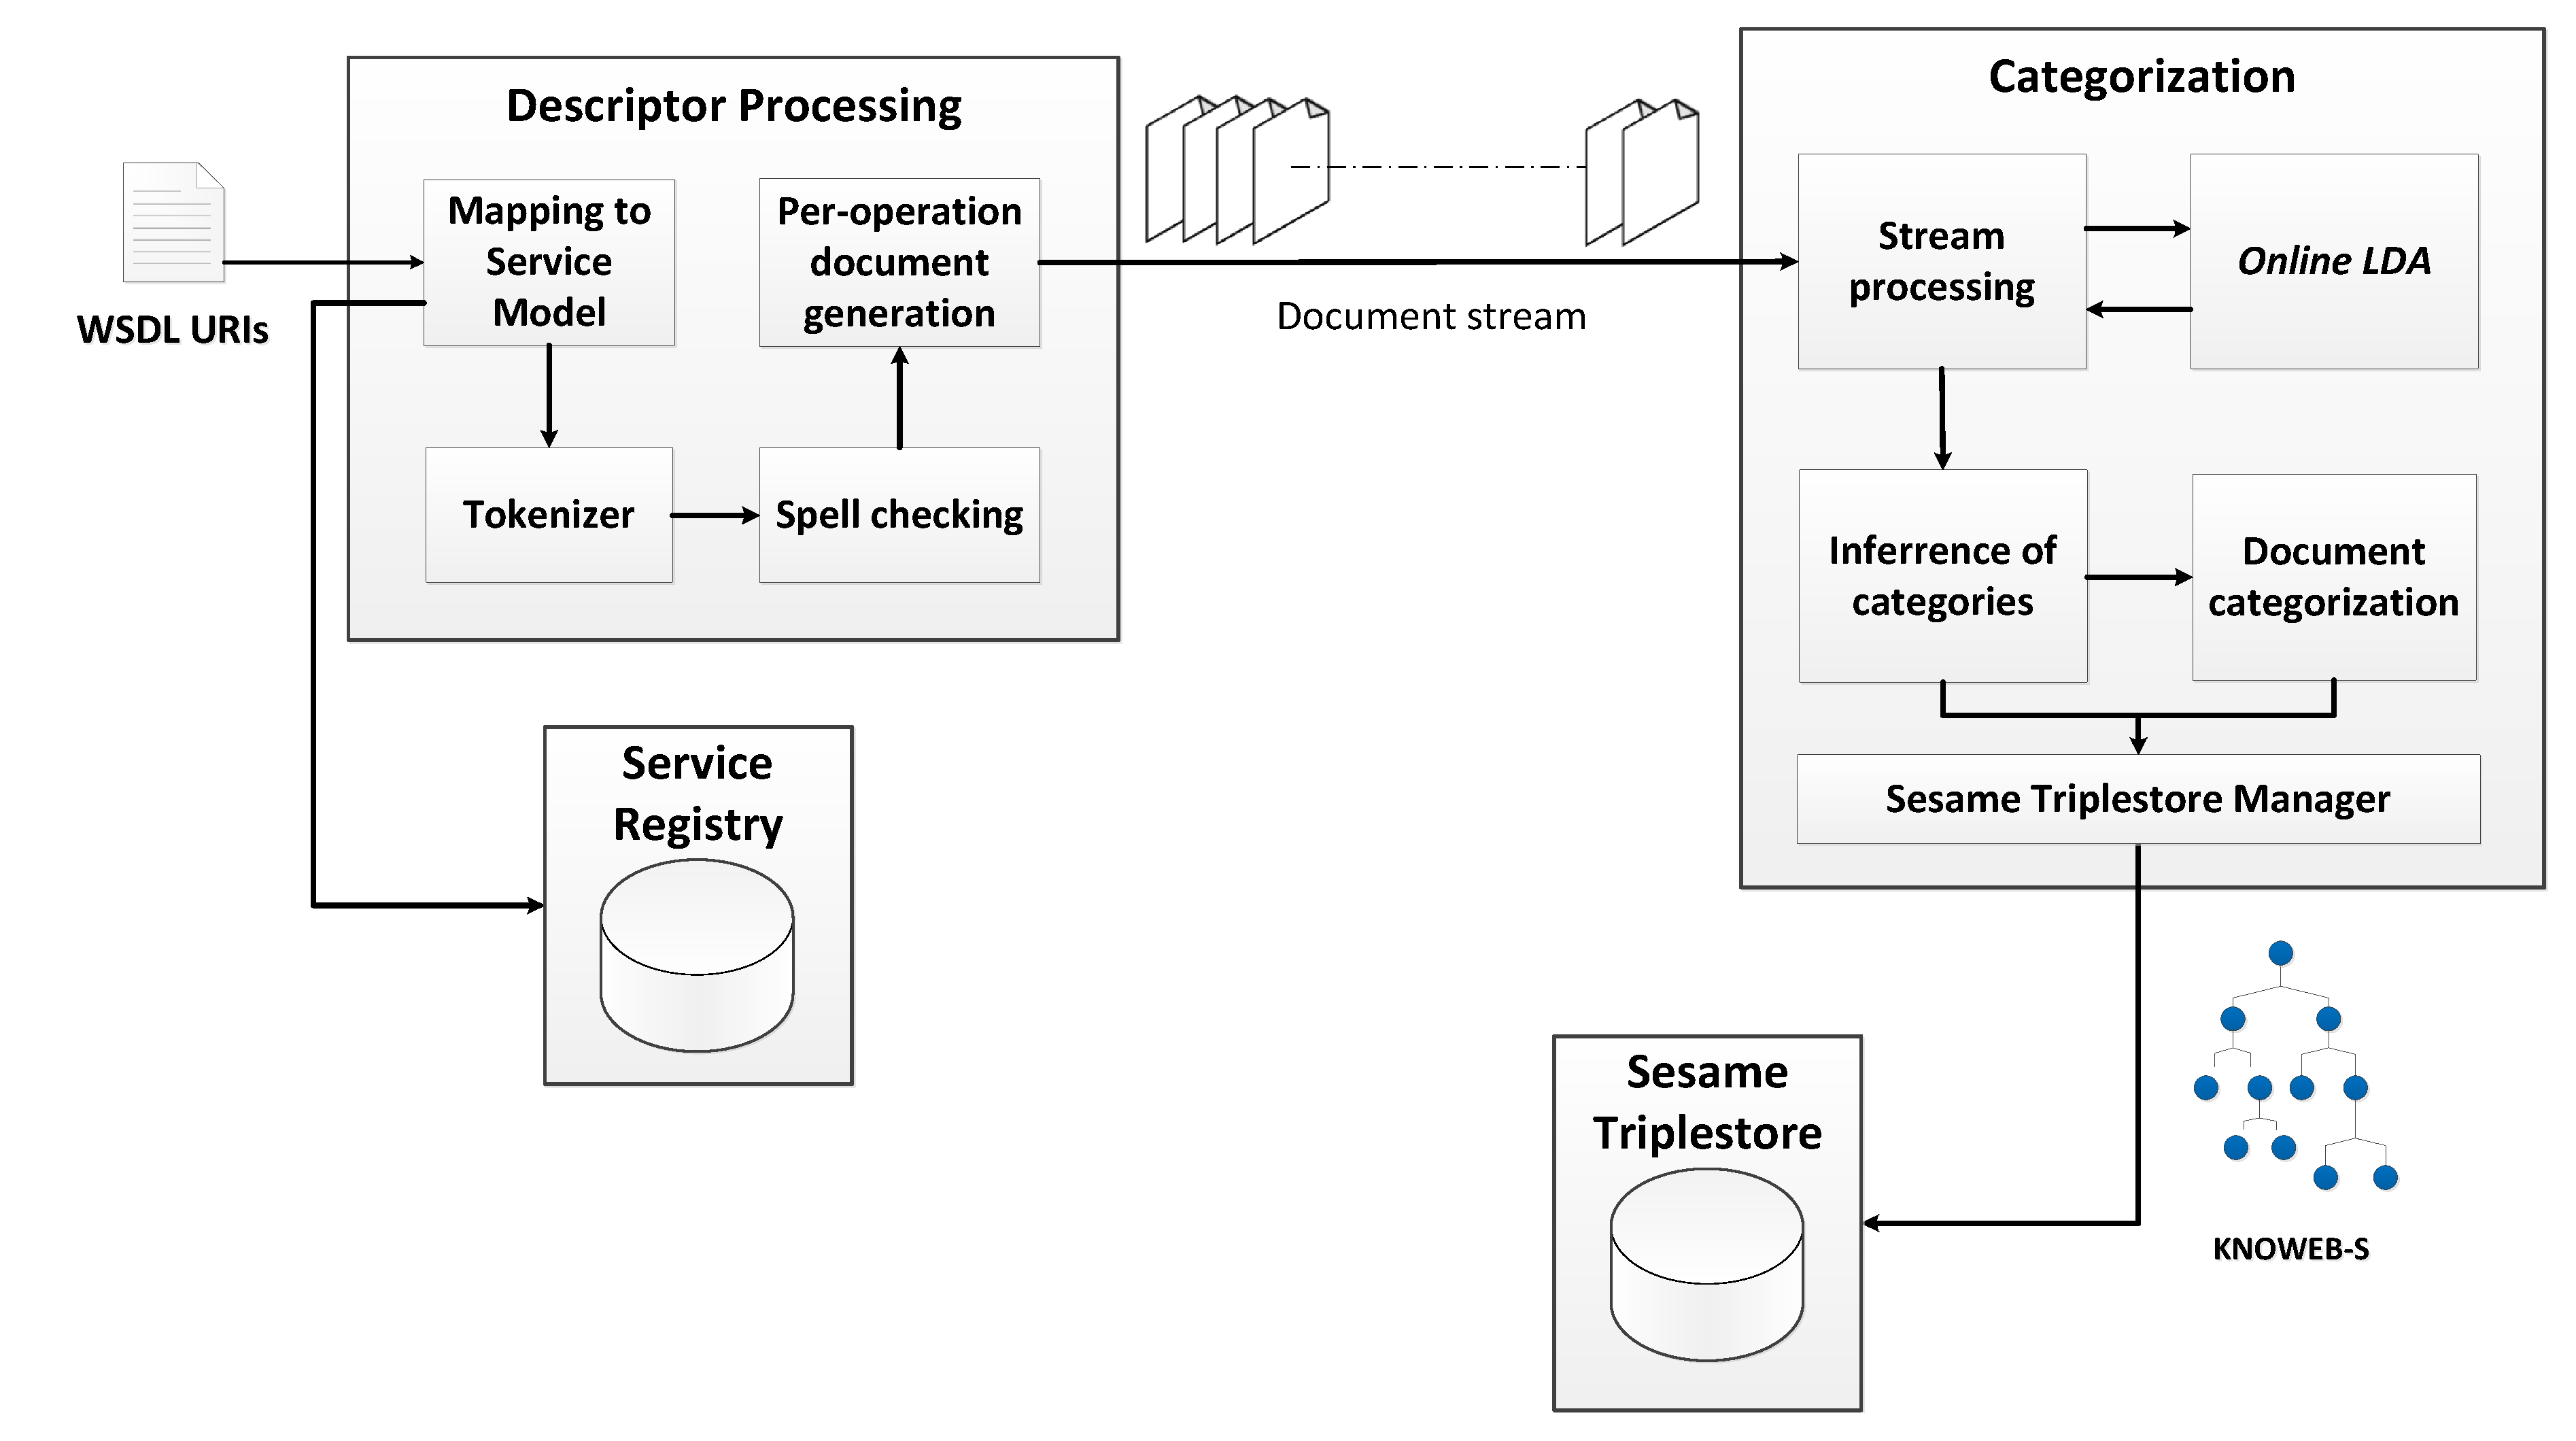
\includegraphics[scale=0.18]{images/prototype-architecture}

\caption{Architecture of Topicalizer.}
\label{prototype-architecture}
\end{center}
\end{figure}


Each one of the components comprising the architecture of Topicalizer are described below:
\begin{itemize}

\item \emph{Descriptor processing}: this module of the architecture is in charge of reading the list of WSDL URIs, accessing each descriptor via HTTP request, loading it into memory, mapping it into the SOAP service model defined in section \ref{subsub:soap} (see Figure \ref{wsdl-Simplified}) and storing the mapped information into a service registry. Once these initial procedures have been performed, this module applies tokenization and spell checking techniques---described in section \ref{subsub:Service-documentation-cleaning}---on the content of each descriptor and finally, for every operation of the processed descriptor it generates a document in plain text containing: (\emph{i}) the operation name, (\emph{ii}) its description in natural language, (\emph{iii}) the name of the service it belongs to, and (\emph{iv}) its input/output parameters. This module was implemented in Java, using its persistence API (JPA) and the \emph{EasyWSDL} library for WSDL manipulation \footnote{Available at: \href{http://
easywsdl.ow2.org/}{http://easywsdl.ow2.org/}}.

\item \emph{Service registry}: consists of a relational database, implemented in MySQL. The entity-relationship model of this database matches the service model described in section \ref{subsub:soap}. 

\item \emph{Categorization}: this component receives the stream of documents generated by the descriptor processing module, then splits it in small-sized batches and delivers them to the implementation of online LDA, which is based on an adaptation of an existing application developed by Matthew D. Hoffman, one of the authors of the mentioned algorithm \cite{Hoffman:2010}. Once the processing of the stream of documents is completed, the derived results are interpreted for establishing the set of terms that compose each category---task performed by the \emph{inference of categories }sub-module---as well as the group of documents included in each one of them---which is defined by the \emph{document categorization} sub-module. The derived arrangement of categories, documents and terms, is mapped into the KNOWEB-S data model and stored into a RDF triplestore provided by the \emph{Sesame} openRDF framework \footnote{Available at: \href{http://www.openrdf.org/index.jsp}{http://www.openrdf.org/index.jsp}}. This 
component of the architecture was developed in Python, using the \emph{numpy}, \emph{urllib2} and \emph{httplib2} libraries.

\item \emph{Sesame Triplestore}: It is an HTTP repository for RDF triples, hosted in an Apache Tomcat web server. This repository stores the KNOWEB-S taxonomy generated by the previous Categorization component. Sesame allows the retrieval and manipulation of the information encoded in KNOWEB-S by using SPARQL queries.
\end{itemize}

The whole prototype is executed by using a bash script, which receives as input the path of a text file containing the list of WSDL URIs. The prototype also generates two documents in \emph{csv} format for specifying: (1) the terms that define each of the identified categories along with their associated relevance value, and (2) the per-document category proportions for each of the processed documents (i.e. SOAP service operations).  
A description of the source code structure of the prototype is available at \href{https://github.com/LeandroOrdonez/Topicalizer}{https://github.com/LeandroOrdonez/Topicalizer}.

For evaluating ou proposal, we have developed a web application \footnote{\textit{TopicalizerBrowser}, available at \href{http://leandrocloud.cloudapp.net:8080/TopicalizerBrowser}{http://leandrocloud.cloudapp.net:8080/TopicalizerBrowser}} (Figure \ref{topicalizer-browser}) intended for human evaluators to visualize and browse through the structure of categories (topics) that pervade a corpus of 200 SOAP service descriptors (which add up to 1328 operations) extracted from the research dataset by Zhang et al. \cite{Zhang:2010}. We asked the evaluators to estimate the coherence of the categorization as well as the relevance of the annotations that our prototype assigns to each individual operation. The procedure that each evaluator followed consist of two steps:

\begin{enumerate}
 \item When assessing a \textit{category}, the evaluator has to assign a name to it, based on its distribution over terms and the operations it contains. Whenever there is no obvious name for a particular category according to the evaluator's judgment, the assigned name is set to ``\textit{NA}'' (i.e. \textit{Not Available})
 \item When assessing an \textit{operation} the evaluator must estimate the relevance of the annotations that the prototype has assigned to it, by approving or disapproving them, and adding new terms that he/she considers the prototype has missed. Figure \ref{evaluated-operation} shows the outcome of performing this step on one web service operation.
\end{enumerate}

We had three evaluators taking part on this process. They went through this procedure on 11 randomly selected categories out of the 40 available, performing the evaluation of 155 operations (that is 15 operations per category).


\begin{figure}[H]
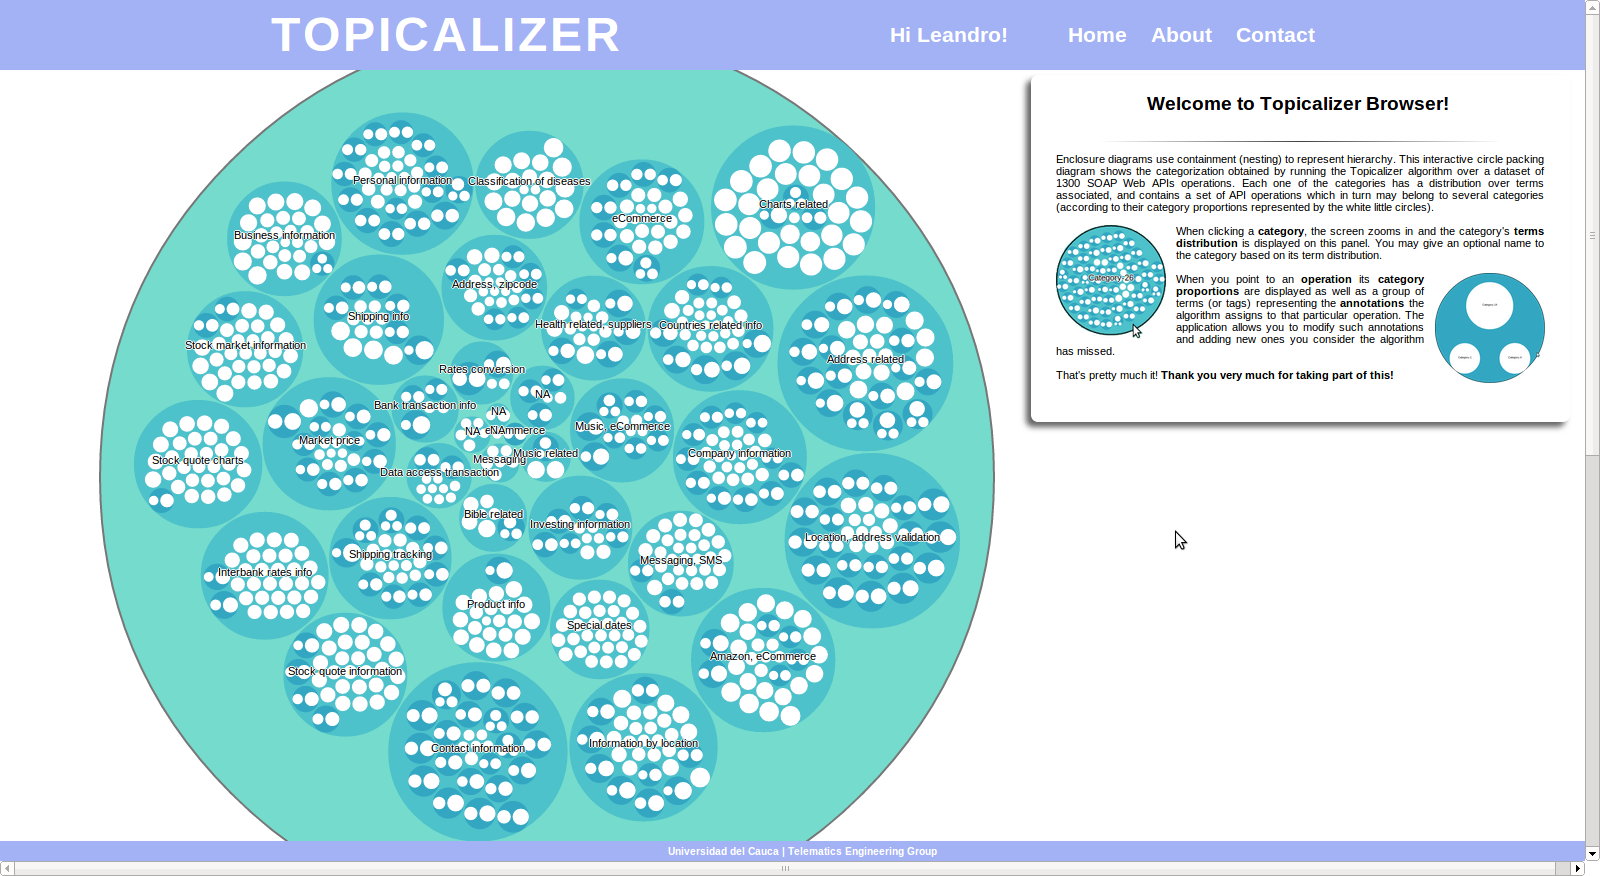
\includegraphics[scale=0.215]{images/TopicalizerBrowser}

\caption{Topicalizer Browser Application}
\label{topicalizer-browser}

\end{figure}

\begin{figure}[H]
\begin{center}
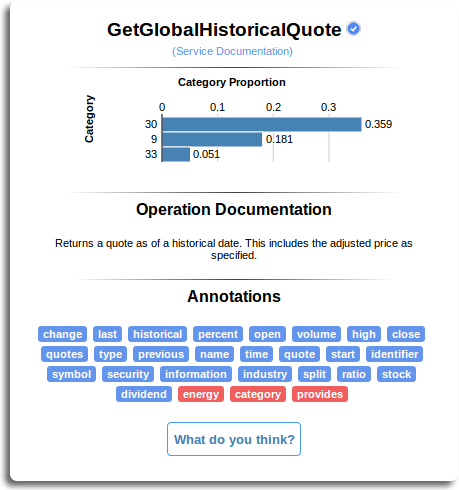
\includegraphics[scale=0.40]{images/EvaluatedOperation}
\caption{Example of a Web service operation annotated by Topicalizer. Blue tags represents the accepted annotations, while red ones are rejected annotations according to the judgment of the evaluator.}
\label{evaluated-operation} 
\end{center}
\end{figure}

Based on the results gathered from this evaluation procedure, we estimate the performance of our proposal by taking three measurements on each of the operations reviewed by the human evaluators: \textit{Precision (P)}, \textit{Recall (R)} and the \textit{Balanced F-measure ($F_1$)}. All three measurements were estimated on each evaluated operation according to the following expressions:

\begin{equation}
P_{op}=\frac{1}{\left|E\right|}\sum_{e=0}^{\left|E\right|}{\displaystyle {\textstyle {\displaystyle \frac{\left|AA_{e}\right|}{\left|RA_{e}\right|+\left|AA_{e}\right|}}}}\label{eq:3}
\end{equation}

\begin{equation}
R_{op}=\frac{1}{\left|E\right|}\sum_{e=0}^{\left|E\right|}{\displaystyle {\textstyle {\displaystyle \frac{\left|AA_{e}\right|}{\left|MA_{e}\right|+\left|AA_{e}\right|}}}}\label{eq:4}
\end{equation}

\begin{equation}
F_{1_{op}}={\displaystyle {\textstyle {\displaystyle \frac{2P_{op}R_{op}}{P_{op}+R_{op}}}}}\label{eq:5}
\end{equation}

where $AA_{e}$, $RA_{e}$ and $MA_{e}$ refer to the sets of \textit{accepted}, \textit{rejected}, and \textit{manual} (non-existent) annotations for evaluator $e$ respectively, while $\left|E\right|$ represents the number of evaluators.

When computing the overall precision, recall and F-measure by summing over all the evaluated operations $op$, the average value of each measurement were respectively 81.48\%, 90.48\% and 85.45\%, outperforming similar approaches, like the one proposed by Falleri et al. in \cite{Falleri:2010}. Figure \ref{p-vs-r} provides a detailed view of the results in terms of the precision and recall of individual operations in the dataset. This graph evidences the capability of our proposal for assigning a \textit{comprehesive} (high recall) set of \textit{relevant} (high precision) annotations to each operation in the dataset since all datapoints lie in the upper right corner of the precision--recall chart.

\begin{figure}[H]
\begin{center}
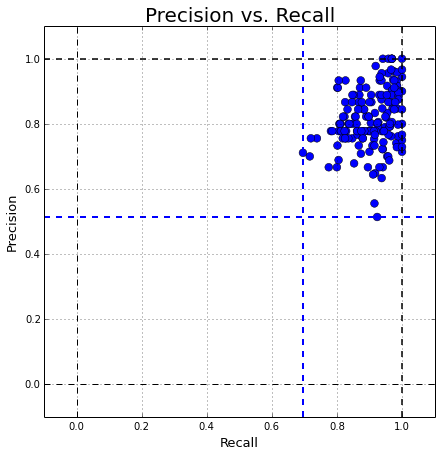
\includegraphics[scale=0.52]{images/PvsR}
\caption{\textit{Precision} vs \textit{Recall} for individual operations in the dataset}
\label{p-vs-r} 
\end{center}
\end{figure}

Figure \ref{prf-vs-c} depicts the average value of precision, recall and F-measure per category. Additionaly this chart shows the set of terms defining each one of the evaluated categories. According to this graph, our system is able to identify semantic related tokens out of the content of web services descriptors, while properly classify service operations within the categories each set of terms defines, with an F-measure ranging from 79.24\% (category 3) to 95\% (category 8).

The results we got from the performance evaluation evidences the feasibility of our approach for classifying and annotating web services supported on probabilistic topic models. It is worth noting that, even though the evaluation was performed on SOAP services, the proposed mechanism would be also suitable for XML-RPC and REST-like web services as long as their documentation is available in a semi-structured format (e.g. HTML documents) so that it can be handled according to the process outlined in section \ref{subsubsec:rpc-rest}.

\begin{sidewaysfigure}
\begin{figure}[H]
\begin{center}
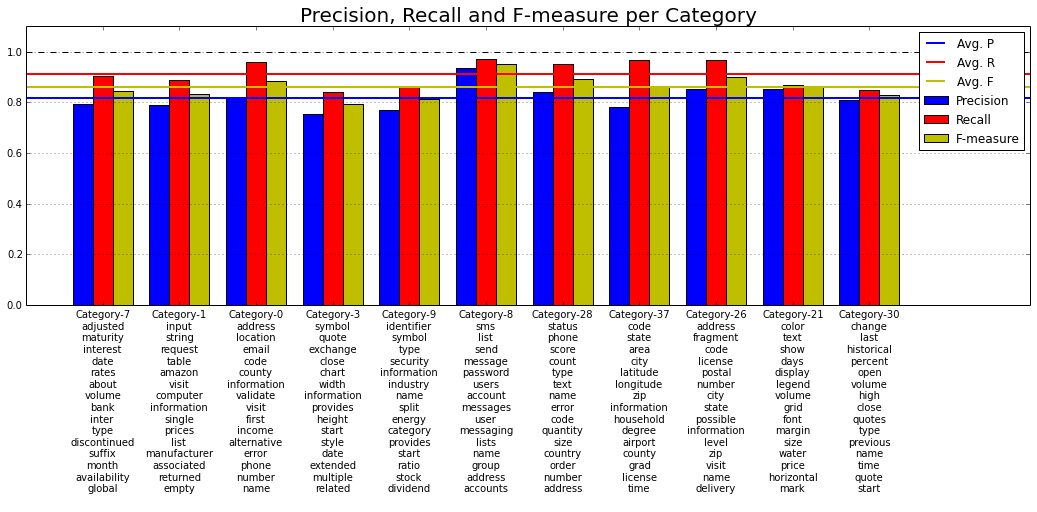
\includegraphics[scale=0.52]{images/PRFvsC}
\caption{\textit{Precision}, \textit{Recall} and \textit{F-measure} per Category. Note that the list of terms defining each category is placed under the Category IDs.}
\label{prf-vs-c} 
\end{center}
\end{figure}
\end{sidewaysfigure}




\section{Discussion and Conclusions}
\label{sec:discussion_conclusions}

\noindent This report documents the activities performed during my research internship at the Multimedia Lab group from Ghent University in the context of the master thesis entitled \textquotedblleft{}\emph{Automated semantic annotation of services on the Web}\textquotedblright{}.

A literature review conducted during the research stay, revealed the benefits of adopting the REST architectural style for building scalable distributed hypermedia systems, like the Web itself. Thanks to the HATEOAS principle of the REST uniform interface, it is possible for automated agents to carry out processes of discovery and composition of services by leveraging the hypermedia controls included in resources representations-- a dynamic that emulates the way humans browse the web---. One of the goals of the Semantic Web consists precisely in enabling computers to understand the underlying meaning of resources, so that they are able to autonomously perform service discovery, invocation and composition. This way, implementing distributed systems that adopt the REST architectural style, turns out to be a practice aligned with the realization of the Semantic Web. However, recent studies has shown that despite the apparent spread of REST services/APIs on the Web, the HATEOAS principle is in most of the cases neglected or misinterpreted.

Bearing this limitation in mind, the research work partially documented in this report, proposes an approach that leverages on existing Web services and their associated documentation sources for generating a knowledge representation which captures the semantics that defines them, in a machine readable format. Such a knowledge representation allows to arrange the services into an structure that reveals semantic relationships among them.

Given a characterization based on the Richardson's maturity model for web services \cite{Richardson:2008}, in this work three types of services are discriminated: SOAP, XML-RPC and REST. For each kind of services we analyze their associated documentation sources to define which information is relevant for setting up the above knowledge representation, as well as the procedure for extracting such information.

The knowledge representation is derived by applying an online variant of the LDA topic model on the information extracted from different Web services documentation sources. This model allows deducing a set of categories that cluster semantically-related service operations and resources. The derived structure of categories is specified by using a standard format based on the RDF data model, and stored into an RDF triplestore.

Finally, the proposed techniques supported the implementation of a prototype for categorizing a set of operations included in SOAP services available online. The results that the developed prototype delivers are promising, however an experimental evaluation that allows to objectively estimate the precision of the generated categorization is still required. This way two main steps have to be done: first, extending the implemented prototype for supporting REST and XML-RPC service documentation analysis, and lastly, perform the experimental assessment of the approach.  

\bibliographystyle{ieeetr}
\bibliography{references}
%\input{references}
%\begin{thebibliography}{9}                                                                                                %
%\bibitem {KarelRektorys}Rektorys, K., \textit{Variational methods in Mathematics,
%Science and Engineering}, D. Reidel Publishing Company,
%Dordrecht-Hollanf/Boston-U.S.A., 2th edition, 1975
%
%\bibitem {Bertoti97} \textsc{Bert\'{o}ti, E.}:\ \textit{On mixed variational formulation
%of linear elasticity using nonsymmetric stresses and displacements}, International
%Journal for Numerical Methods in Engineering., \textbf{42}, (1997), 561-578.
%
%\bibitem {Szeidl2001} \textsc{Szeidl, G.}:\ \textit{Boundary integral equations for
%plane problems in terms of stress functions of order one}, Journal of Computational and
%Applied Mechanics, \textbf{2}(2), (2001), 237-261.
%
%\bibitem {Carlson67}  \textsc{Carlson D. E.}:\ \textit{On G\"{u}nther's stress functions
%for couple stresses}, Quart. Appl. Math., \textbf{25}, (1967), 139-146.
%\end{thebibliography}
\end{document}